\section{Architecture}
\label{sec:cod_architecture}
This section describes the implementation of the COD module, which implements the parameterized function $f_{\theta}$. 
\newline 
As described in the previous paragraph this function must generate a set of object category agnostic bounding-boxes $\left\{ bb^{j}_{t} | j \in C \right\}$, where $ bb^{j}_{t}\in \mathcal{R}^{4}$ is a vector of 4 elements containing the coordinates of the bounding-box defined as the upper-left (ul) and bottom-right (br) corners $\left[x^{ul}, y^{ul}, x^{br}, y^{br}\right]$. To each predicted bounding-box is assigned a class that refers to the semantic attribute associated with the object for a given command. 
The bounding-boxes are generated by taking in input:
\begin{itemize}
    \item \textit{Agent Observation},  $o^{a}_{t} \in \mathcal{R}^{H \times W \times 3}$, which is a RGB image which represents both the state of the agent as well as the state of the environment.
    \item \textit{Demonstrator Command}, $c_{m_{i}} \in \mathcal{R}^{T \times H \times W \times 3}$, which is a sequence of $T$ frames sampled from a video of a demonstrator performing the requested task.
\end{itemize}

In the field of Computer Vision, Object Detection is a well established and extensively researched problem, with modern techniques achieving high performance in both detection and classification tasks. However, the methods used in previous work \cite{jiang2023vima, zhu2023viola} are not applicable here. The objective in this case is not to detect all objects in the scene, but rather to identify ``target locations", which can vary depending on the specific task at hand (Figure \ref{fig:example_of_bb}). Additionally, the method must be \textbf{category-agnostic}, meaning it does not need to answer the question, ``What category does the object belong to?" Instead, the primary goal is to determine, ``Where is the target object located?" This allows the approach to be easily adapted to scenarios involving multiple object categories.


To solve the given problem, inspiration was drawn from another well-known task in computer vision, namely, ``Visual Question Answering'' \cite{perez2018film}. In this task, the system generates an answer to a given query (e.g., a textual question) based on an input image. What distinguishes this approach is its ability to \textbf{selectively focus on specific segments of the image}, guided by the content of the question, as illustrated in Figure \ref{fig:film_attention}.


The proposed approach is rooted in the concept that, similar to the architecture presented in \cite{perez2018film}, which directs attention to specific regions of an image in response to input queries, our model aims to achieve a similar capability. Specifically, the model is designed to focus on certain regions of the image based on the task command $c_{m_{i}}$. The proposed architecture is shown in Figure \ref{fig:cod}.
\begin{figure}[t]
    \centering
    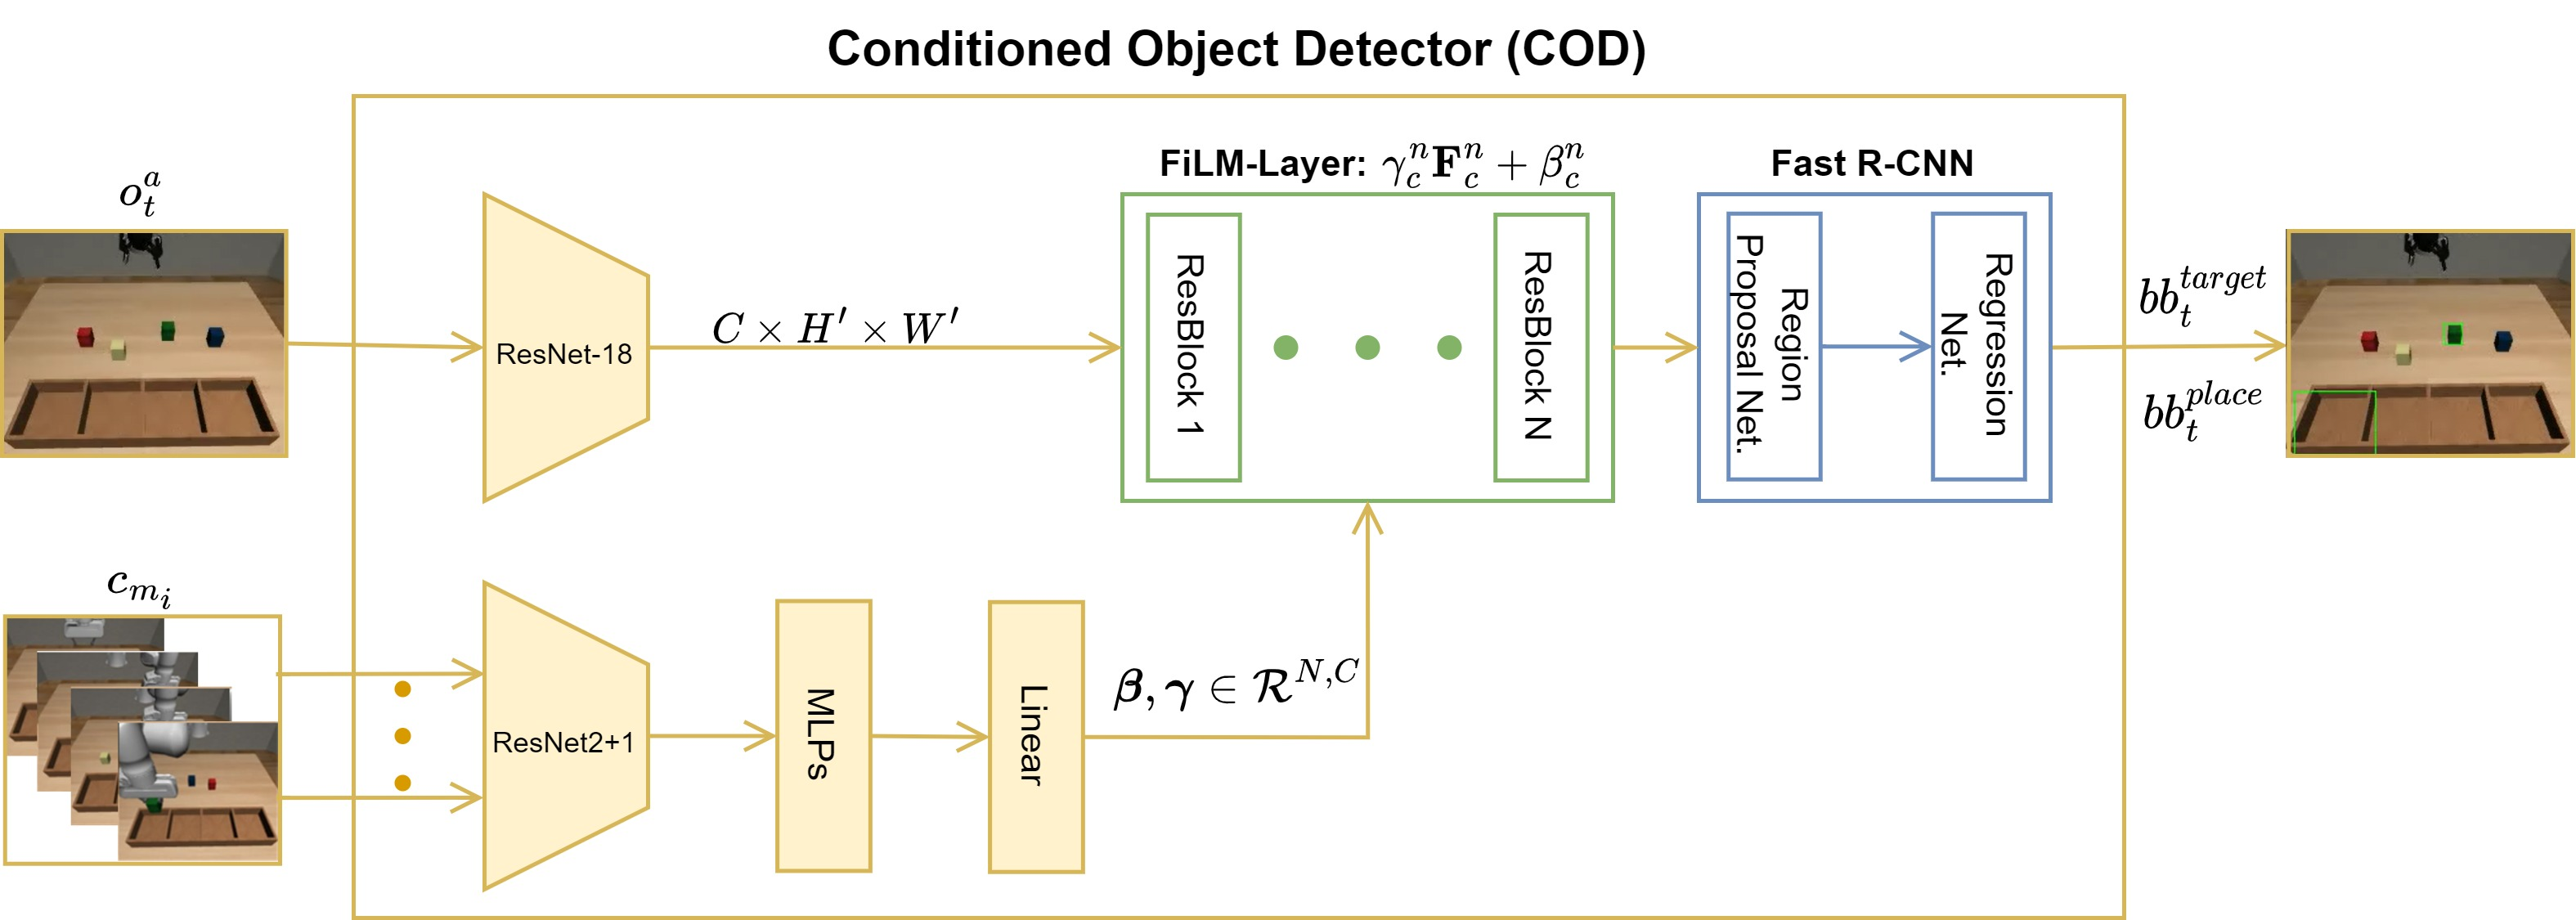
\includegraphics[width=1.0\textwidth]{figures/images/ch2/cod.jpg}
    \caption{The proposed \textit{Conditioned Object Detector} architecture takes as input the pair $(o^{a}_{t}, c_{m_{i}})$, where $o^{a}_{t}$ represents the agent observation and $c_{m_{i}}$ represents the demonstration frames. The agent observation is encoded using ResNet-18, while the demonstration frames are encoded through ResNet2+1. The FiLM conditioning layer is employed to inject information from the command $c_{m_{i}}$ into the feature maps extracted from the observation. Finally, Fast R-CNN generates the bounding boxes based on the conditioned input.}
    \label{fig:cod}
\end{figure}


The architecture consists of the following modules:
\begin{itemize}
    \item \textit{ResNet-18} \cite{resnet}, used as a feature extractor for the agent observation $o^{a}_{t}$, represented as an RGB image.
    \item \textit{ResNet2+1} \cite{resnet21}, employed as a feature extractor for the command description $c_{m_{i}}$. This description consists of 4 frames sampled from the demonstration video. The architecture is designed to extract both spatial and temporal features, which are then flattened and passed through a Multilayer Perceptron (MLP) network.
    \item The FiLM-Layer, as introduced in \cite{perez2018film}, is responsible for integrating the features from both the agent observation and the command description. It modulates the $c^{th}$ activation through a feature-wise affine transformation, expressed as in Formula \ref{eq:film_eq}. Here, $\gamma_{c}$ and $\beta_{c}$ are parameters generated by the linear module based on the input.
    \item \textit{Fast R-CNN} \cite{fastrcnn}, a two-stage anchor-based object detector, is used to predict the bounding box position based on the feature maps generated by the preceding module.
\end{itemize}

The entire architecture is trained using the classic object-detection loss function $\mathcal{L} = w_{1}\mathcal{L}_{reg} + w_{2}\mathcal{L}_{cls} + w_{3}\mathcal{L}_{class}$, where:
\begin{itemize}
    \item $\mathcal{L}_{reg}$ is the \textit{L1-loss} function that compares the predicted bounding box offset with the ground truth offset.
    \item $\mathcal{L}_{cls}$ is a \textit{binary cross-entropy loss} that allows the model to learn the difference between foreground and background bounding boxes.
    \item $\mathcal{L}_{class}$ is a cross-entropy loss designed for object classification.
\end{itemize}

Once the architecture has been fully described, we can introduce the experiments conducted to evaluate the proposed model. A detailed explanation of these experiments, along with the results, will be provided in Section \ref{sec:cod_experimental}.
